\section{Experiment 2}
In this experiment we would like to experimentally verify that our simulation gets more accurate as we increase the mesh resolution. We will do this by applying light gravitational force to a cantilever beam fixed to a wall. We then measure the position of a lowest hanging vertex as we increase the mesh resolution. In the real world gravity would be applied to all molecules, and so our expectation is the measured position converge towards some fixed value as the simulation gets more realistic with more nodes. Our initial grid resolution will be 12x4, and we will then increase the mesh resolutions in multiples of this initial resolution. The results can be seen in \autoref{positions}.
\begin{figure}
	\centering
	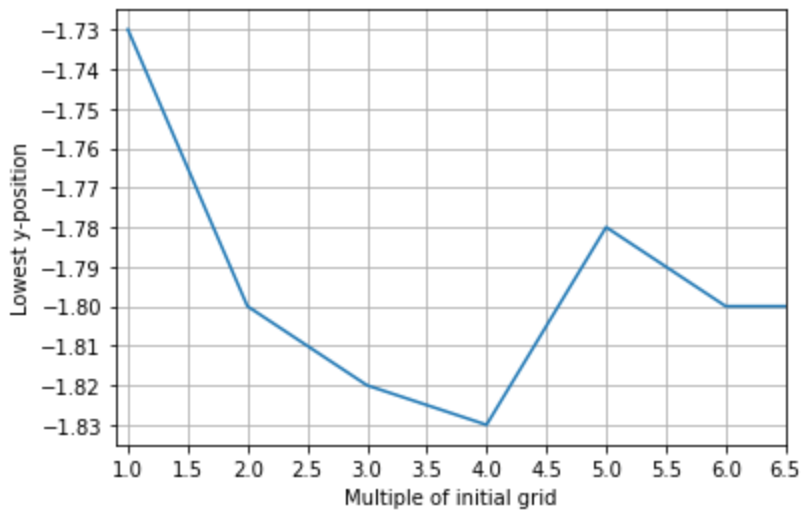
\includegraphics[width=0.9\linewidth]{Materials/positions}
	\caption{Lowest vertex position of the simulation measured for different mesh resolutions.}
	\label{positions}
\end{figure}

\subsection{Discussion of results}
In the beginning we see the lowest positions changes quite a lot as we make the grid finer, but towards the end it seems the lowest position converges towards $-1.8$. This matches our expectation about fine mesh resolutions would converge towards a fixed value. We thus conclude our discretization of how the forces are applied is correct.